\chapter{Implementation}

\section{Introduction}
This chapter presents the realization of MapIT in the source code. It is intentionally project-specific: the implementation is not described as a generic web application, but as a Next.js 15 and Express.js platform that serves IT infrastructure documentation, incident tracking, asset inventory, relationship mapping, search, reporting, and access control.

\section{Technical Stack and System Architecture}
\subsection{Monorepo structure}
MapIT is organized as a workspace-based monorepo. The main workspace folders are:
\begin{itemize}
	\item \texttt{apps/api}
	\item \texttt{apps/web}
	\item \texttt{apps/mobile}
	\item \texttt{packages/shared}
\end{itemize}
The most important root scripts are:
\begin{itemize}
	\item \texttt{dev:api}, \texttt{dev:web}, \texttt{dev:mobile}
	\item \texttt{typecheck}, \texttt{test:api}, \texttt{smoke:frontend}, \texttt{ci}
\end{itemize}
This structure is important because it separates the operational backend, the browser interface, and the mobile prototype while keeping the project coherent.

\subsection{Web implementation stack}
The web interface uses Next.js 15 with the App Router, React 19, and TypeScript in strict mode. The styling relies on Tailwind CSS 3 and a utility-driven component system, while the state management layer uses Zustand. API calls are made through an Axios client with a 10-second timeout, \texttt{withCredentials} enabled, and a response interceptor that redirects to \texttt{/login} on HTTP 401. The project also uses Lucide icons, React Hook Form, Zod, SWR, TanStack React Query, and Recharts where the UI needs them.

\subsection{Backend implementation stack}
The backend is built on Express 5, Prisma ORM, PostgreSQL, JSON Web Tokens, and ldapjs for Active Directory authentication in production. The server structure is modular: each domain has its own route file under \texttt{apps/api/src/modules/}. There are dedicated modules for authentication, incidents, documents, dashboard summaries, assets, problems, relationships, search, reports, notifications, settings, and administration.

\subsection{Data and persistence layer}
The Prisma schema defines the real MapIT data model. The main entities include:
\begin{itemize}
	\item \texttt{User}, \texttt{Incident}, \texttt{Document}, \texttt{Asset}, \texttt{Problem}, \texttt{Relationship}
	\item \texttt{Role}, \texttt{Permission}, \texttt{UserRole}, \texttt{RolePermission}, \texttt{UserPermission}
	\item \texttt{UserSettings}, \texttt{AuditLog}, and \texttt{IncidentKnowledgeFeedback}
\end{itemize}
This is the persistence layer that makes the platform suitable for technical documentation rather than only for temporary user input.

\section{Authentication and Access Control}
\subsection{Login flow}
The login route accepts a username and password, authenticates against Active Directory through ldapjs when the application is not in development mode, and supports test credentials when \texttt{DEV\_MODE=true}. After successful authentication, the user is upserted in the database, assigned a default role, and issued a JWT valid for one day. The web login page posts to \texttt{/api/auth/login} and then redirects the user to the dashboard.

The login interface is shown in Figure~\ref{fig:ui-login}.

\begin{figure}[H]
	\centering
	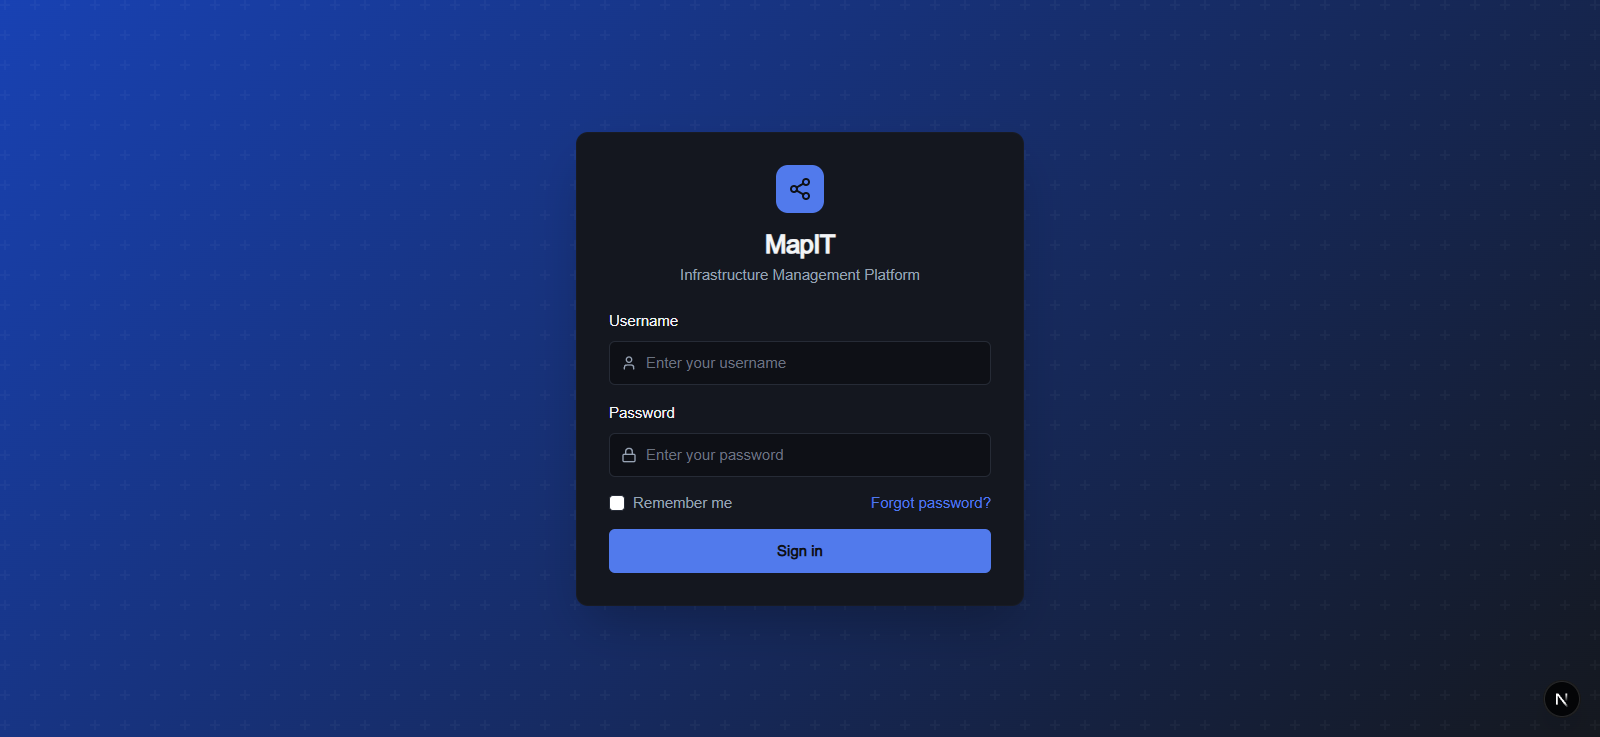
\includegraphics[width=0.9\textwidth]{figures/screenshots/login_page.png}
	\caption{Login page}
	\label{fig:ui-login}
\end{figure}

\subsection{Session and proxy handling}
The frontend does not talk directly to the backend hostname. It sends requests to the Next.js proxy path \texttt{/api/backend/[...path]}, which forwards the browser traffic to the API while keeping the public web application same-origin. The auth store also checks \texttt{/api/auth/session} to determine whether the session is still valid. This is a practical implementation pattern for a secure and deployment-friendly web application.

\subsection{Role-based and permission-based access control}
MapIT goes beyond a simple admin/viewer split. The backend bootstraps permissions and role templates for Admin, Manager, Operator, and Viewer, and it supports user-specific permission overrides. Middleware functions such as \texttt{requireAuth}, \texttt{requireRole}, and \texttt{requirePermission} protect the API. The permission catalog includes fine-grained actions, for example:
\begin{itemize}
	\item \texttt{asset:create}, \texttt{incident:status:update}, \texttt{incident:assign}
	\item \texttt{relationship:create}, \texttt{report:view}, \texttt{settings:update-any}
	\item \texttt{user:manage}, \texttt{permission:manage}
\end{itemize}

Figure~\ref{fig:ui-access-control} illustrates the access-control administration interface used to manage these permission assignments.

\begin{figure}[H]
	\centering
	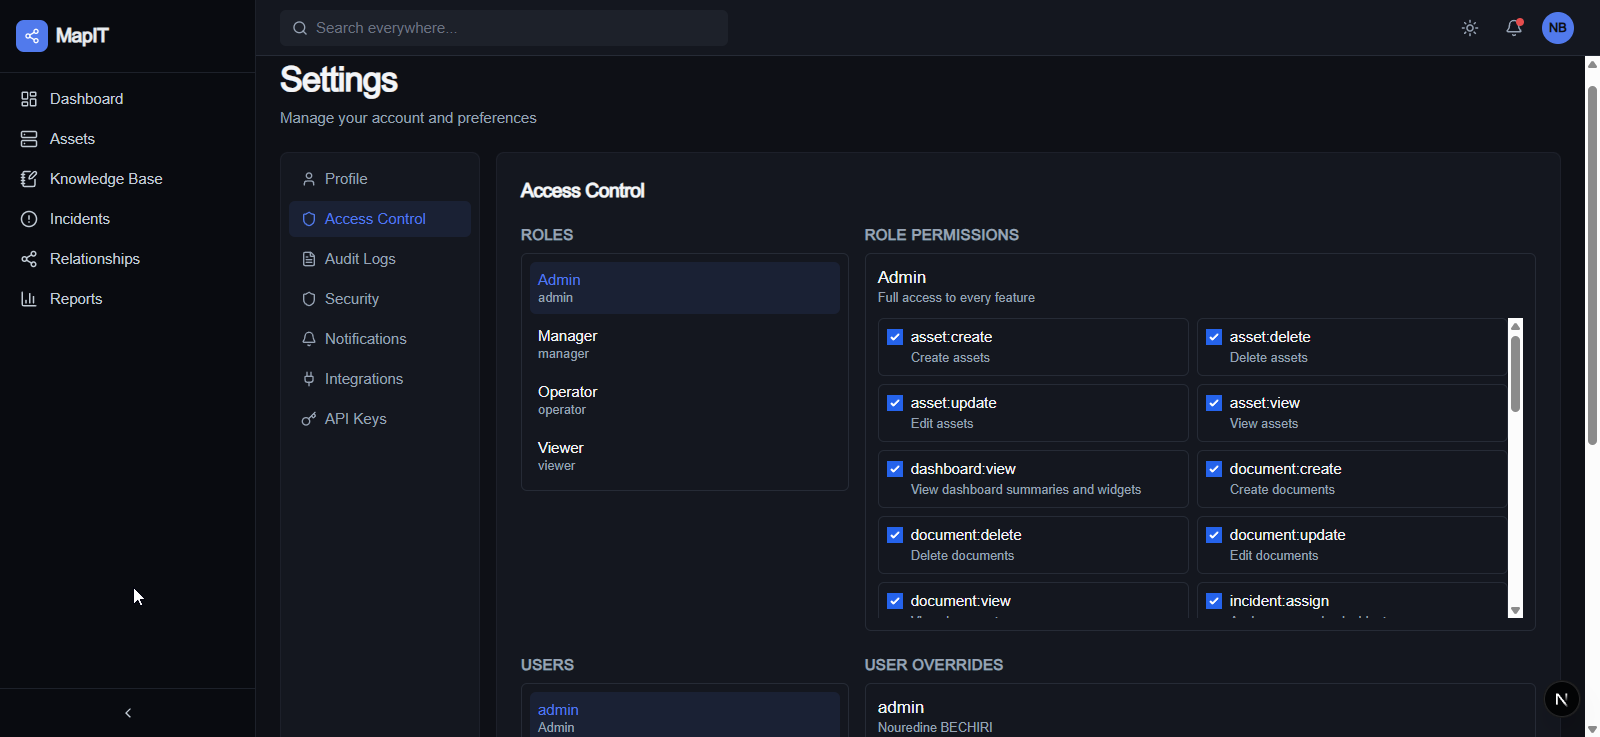
\includegraphics[width=0.95\textwidth]{figures/screenshots/access_control.png}
	\caption{Access control management interface}
	\label{fig:ui-access-control}
\end{figure}

\section{Backend Modules and Business Functions}
\subsection{Incidents}
The incident module is one of the core components of MapIT. It manages incident creation, status transitions, assignment, and knowledge suggestions. The model uses the statuses \texttt{OPEN}, \texttt{IN\_PROGRESS}, \texttt{BLOCKED}, \texttt{RESOLVED}, and \texttt{CLOSED}, together with priorities from \texttt{LOW} to \texttt{CRITICAL}. The detail screen in the web app allows the user to edit the title, description, assigned team, assignee, and status, and it also integrates related knowledge suggestions.

\subsection{Assets and relationships}
The assets module stores infrastructure components such as servers, virtual machines, network devices, storage nodes, and services. The relationship module creates directed connections between assets and returns the graph used by the relationship map page. In the frontend, the map supports dragging nodes, filtering by type, panning, and zooming. This is how MapIT makes infrastructure interdependence visible.

\subsection{Problems and knowledge reuse}
The problems module stores documented problems, affected assets, severity, status, solution text, and resolution dates. This module is the reusable knowledge layer of the application. It is exposed in the Problems page, where users can create, edit, filter, and delete problem entries according to their permissions. The global search module uses these records together with assets, incidents, and documents to produce a unified search result.

\subsection{Search, reports, settings, and audit logs}
The search page performs global search across all knowledge domains. The reports page summarizes assets by type and problems by severity and provides CSV/PDF export. The settings page manages profile data, notifications, theme preferences, access-control administration, and audit-log inspection. The audit trail stores actor, action, resource, and sanitized request metadata so that sensitive operations remain traceable.

The audit trail visualization in Figure~\ref{fig:ui-audit-logs} shows how operational actions remain traceable over time.

\begin{figure}[H]
	\centering
	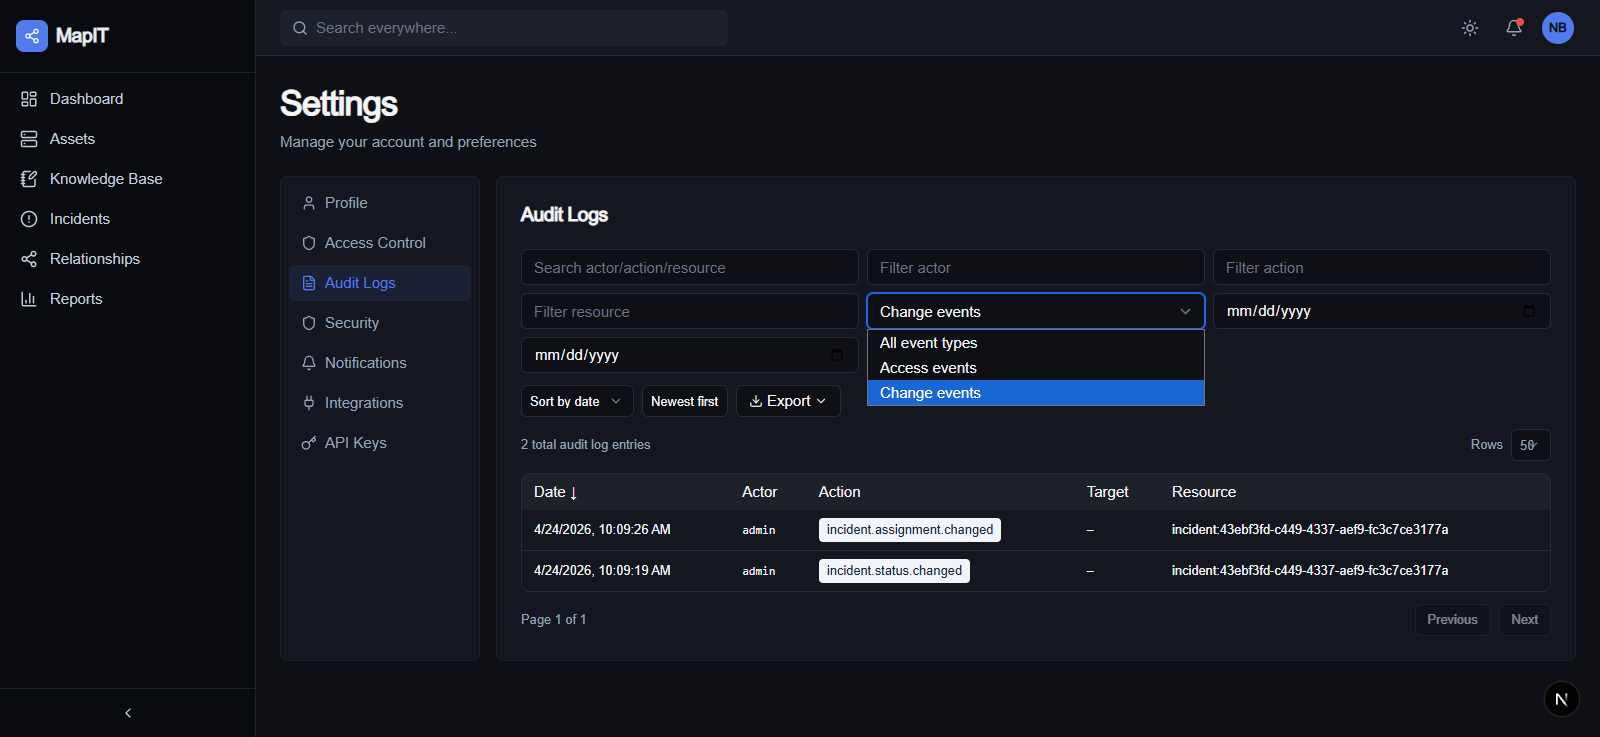
\includegraphics[width=0.95\textwidth]{figures/screenshots/audit_logs.png}
	\caption{Audit logs interface}
	\label{fig:ui-audit-logs}
\end{figure}

\section{Realized User Interfaces}
\subsection{Login and shared layout}
The login page contains a username field, a password field, inline error feedback, and a sign-in button. After authentication, the application redirects to the dashboard. The authenticated pages share a sidebar layout, which is used consistently on the dashboard, incidents, assets, problems, relationships, reports, and settings sections.

\subsection{Dashboard}
The dashboard is not a static welcome page. It loads summary data, assets, and problems in parallel and exposes export actions for CSV and PDF generation. The user can navigate from the dashboard to assets or problems directly, which makes it a control center for the infrastructure team.

\begin{figure}[H]
	\centering
	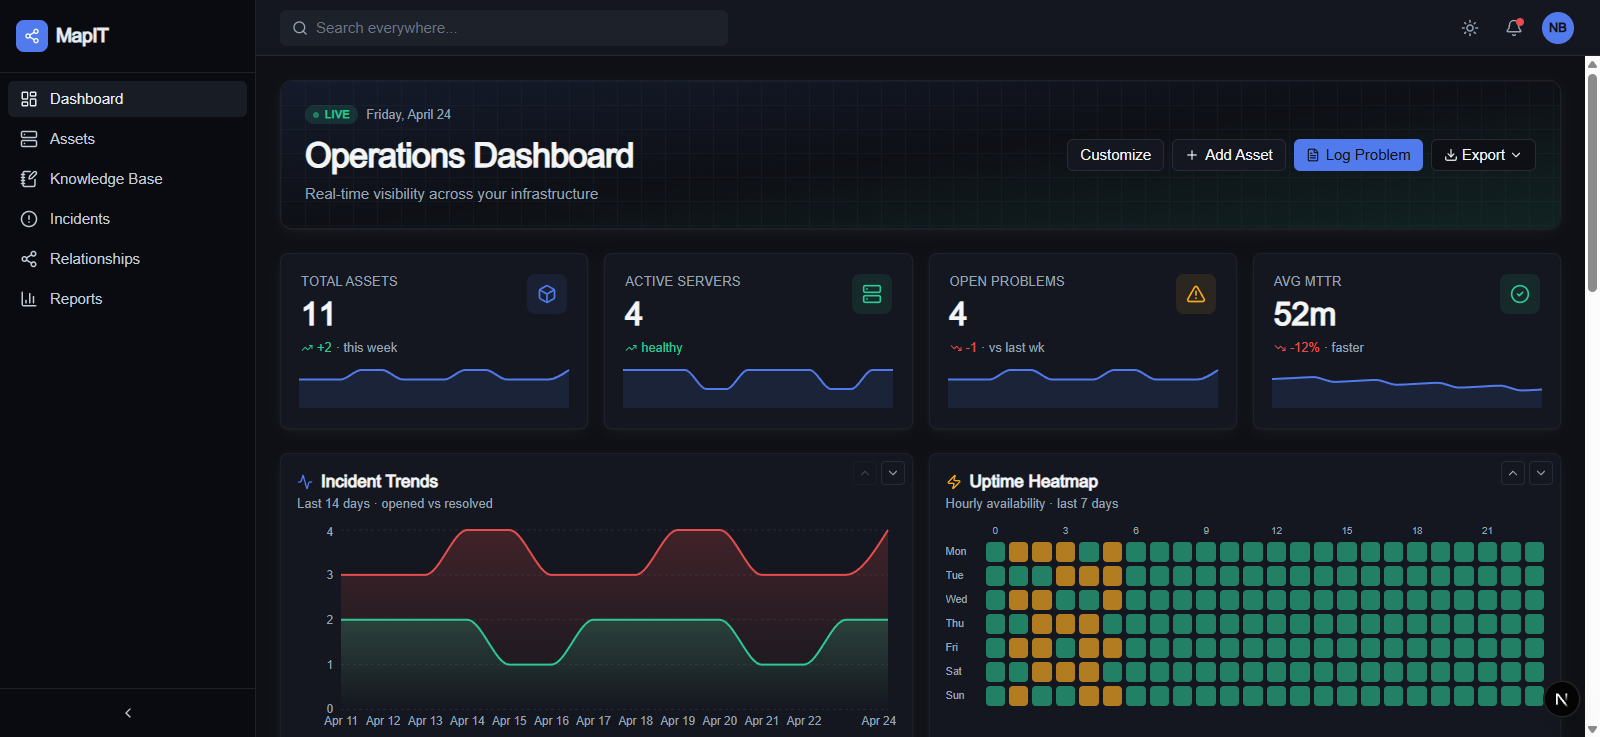
\includegraphics[width=0.95\textwidth]{figures/screenshots/dashboard.png}
	\caption{Dashboard interface}
	\label{fig:ui-dashboard}
\end{figure}

\subsection{Incidents}
The incidents list page supports search by title and description, creation of new incidents, and navigation to incident detail pages. The detail page supports editing, status updates, assignment changes, deletion, and knowledge suggestions. The page also shows status badges and priority badges, which are important for rapid operational reading.

\begin{figure}[H]
	\centering
	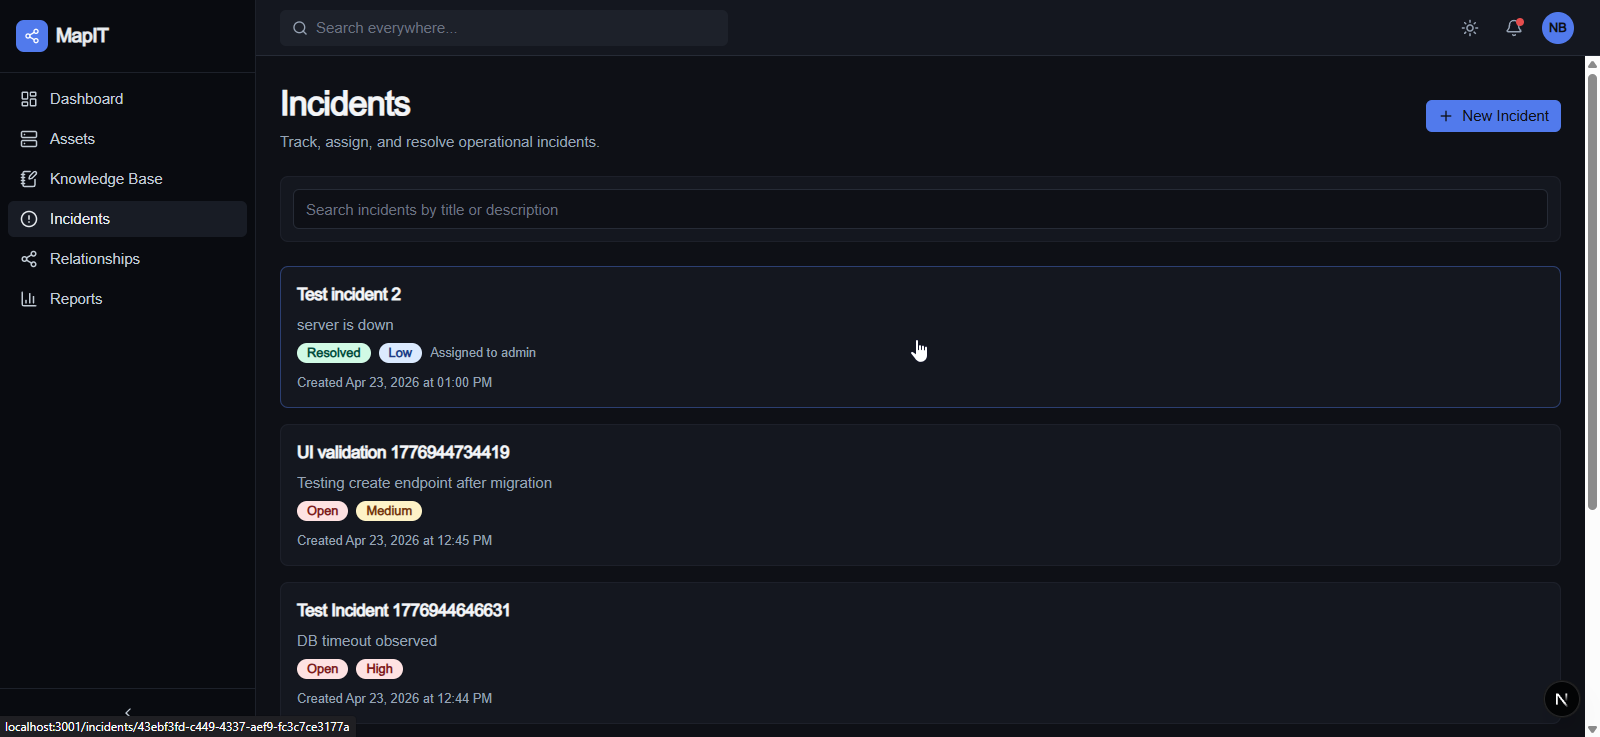
\includegraphics[width=0.95\textwidth]{figures/screenshots/incidents.png}
	\caption{Incidents management interface}
	\label{fig:ui-incidents}
\end{figure}

\subsection{Assets}
The asset inventory page supports filtering, pagination, bulk selection, and an asset creation form that can also create relationships immediately after the asset is saved. The asset detail page shows overview data, related problems, and related assets in separate tabs. The presence of a direct link to the relationship map reinforces the visual nature of the knowledge model.

\begin{figure}[H]
	\centering
	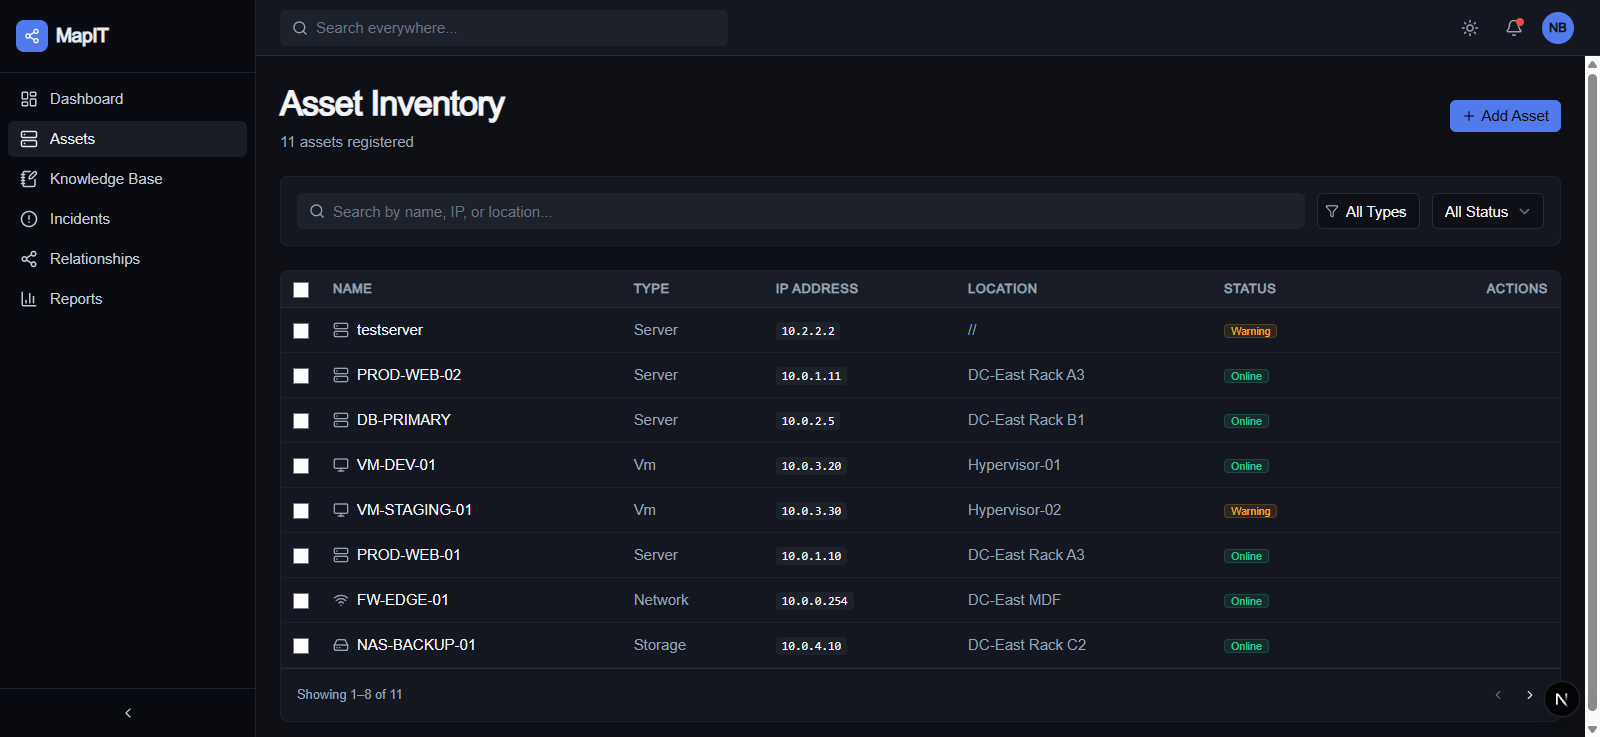
\includegraphics[width=0.95\textwidth]{figures/screenshots/assets.png}
	\caption{Assets inventory interface}
	\label{fig:ui-assets}
\end{figure}

\subsection{Problems, relationships, search, reports, and settings}
The problems page allows the user to manage problem records and associate them with affected assets. The relationships page visualizes the infrastructure graph and supports interactive layout editing. The search page searches across assets, incidents, problems, and documents in one place. The reports page summarizes operational data. The settings page exposes access control, audit logs, security, notifications, integrations, and API-key placeholders.

\begin{figure}[H]
	\centering
	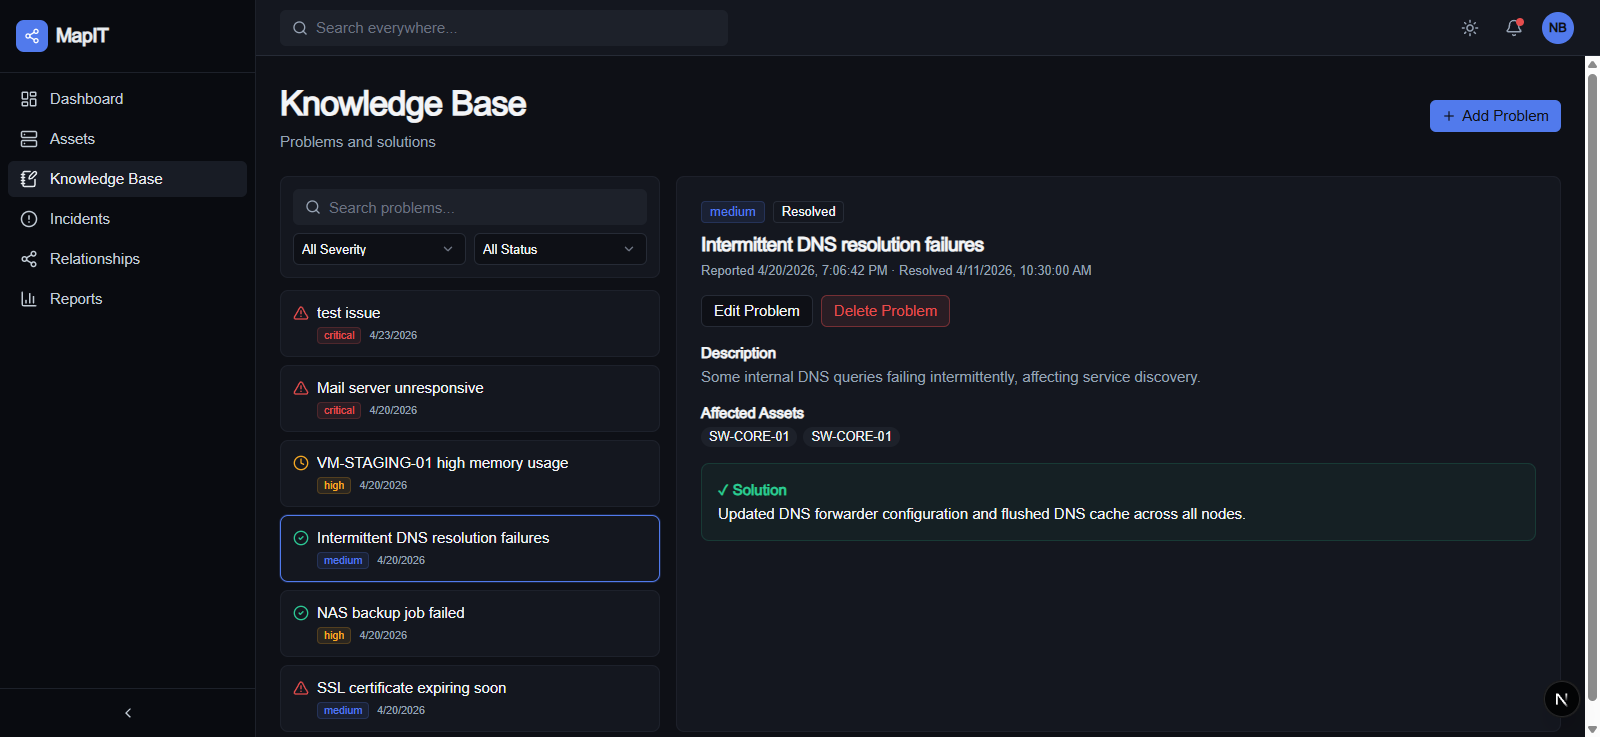
\includegraphics[width=0.95\textwidth]{figures/screenshots/knowledge_base.png}
	\caption{Problem and knowledge base interface}
	\label{fig:ui-knowledge-base}
\end{figure}

\begin{figure}[H]
	\centering
	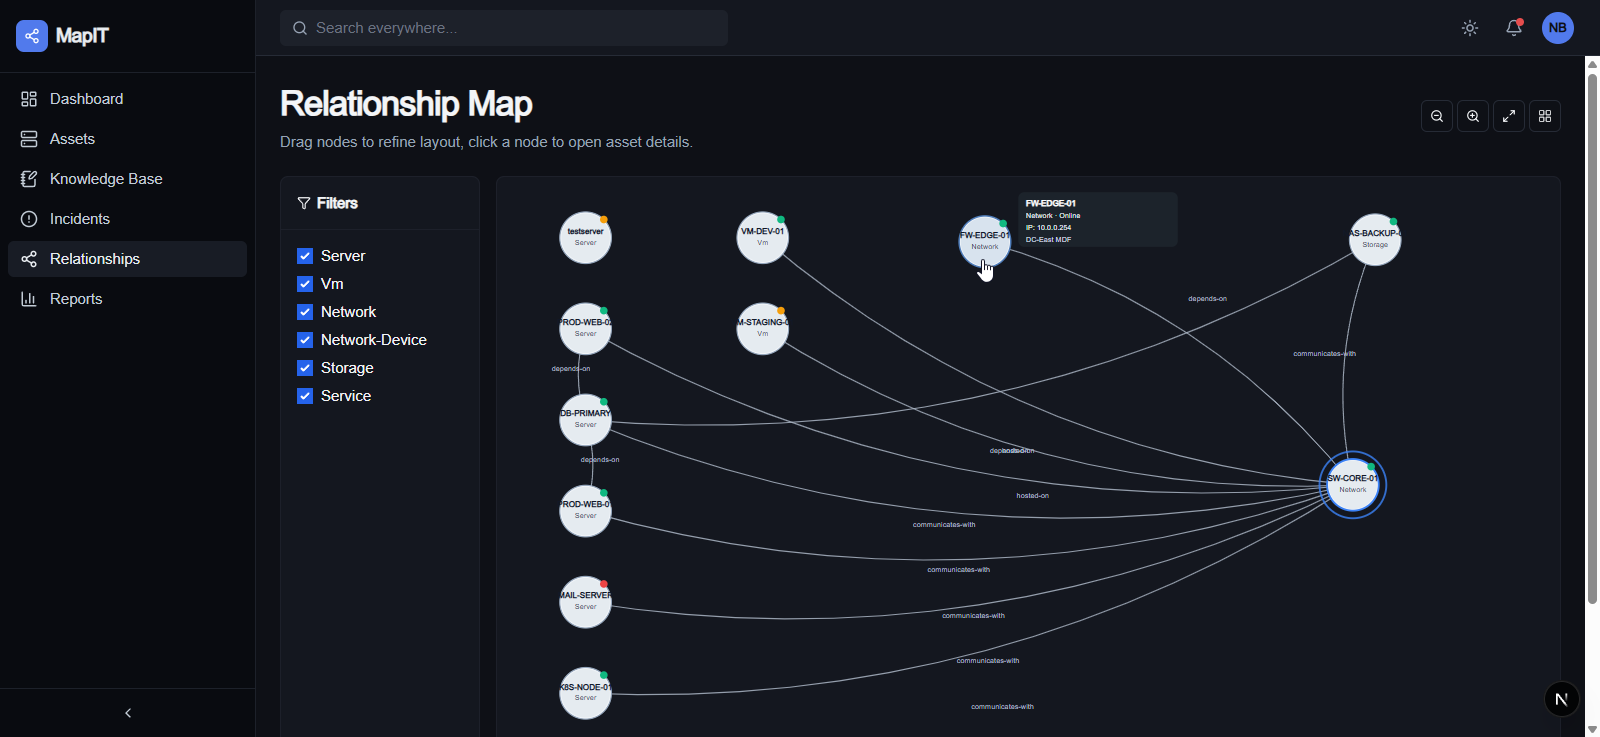
\includegraphics[width=0.95\textwidth]{figures/screenshots/relation_map.png}
	\caption{Relationship map interface}
	\label{fig:ui-relationship-map}
\end{figure}

\begin{figure}[H]
	\centering
	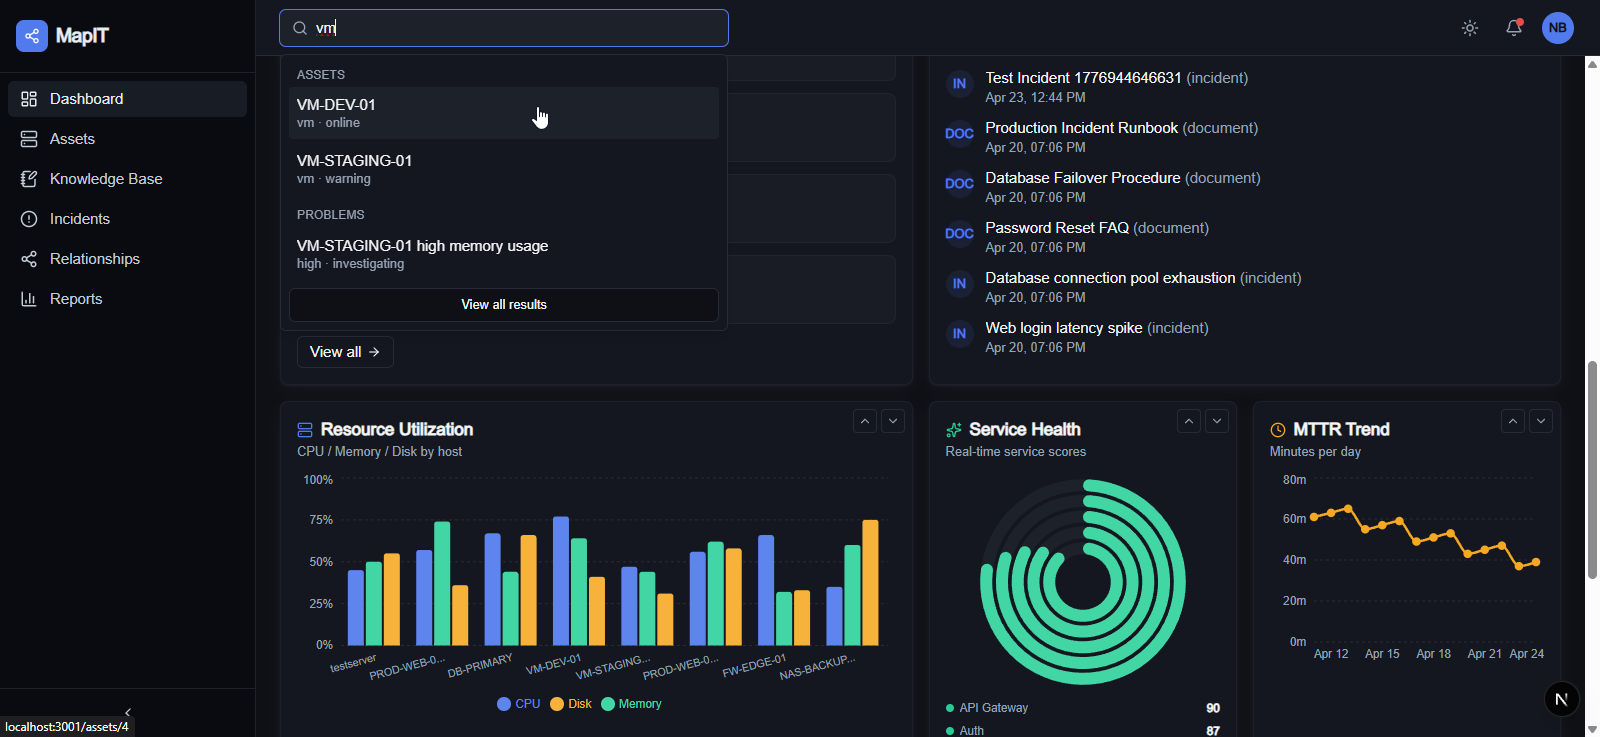
\includegraphics[width=0.95\textwidth]{figures/screenshots/search.png}
	\caption{Global search interface}
	\label{fig:ui-search}
\end{figure}

\begin{figure}[H]
	\centering
	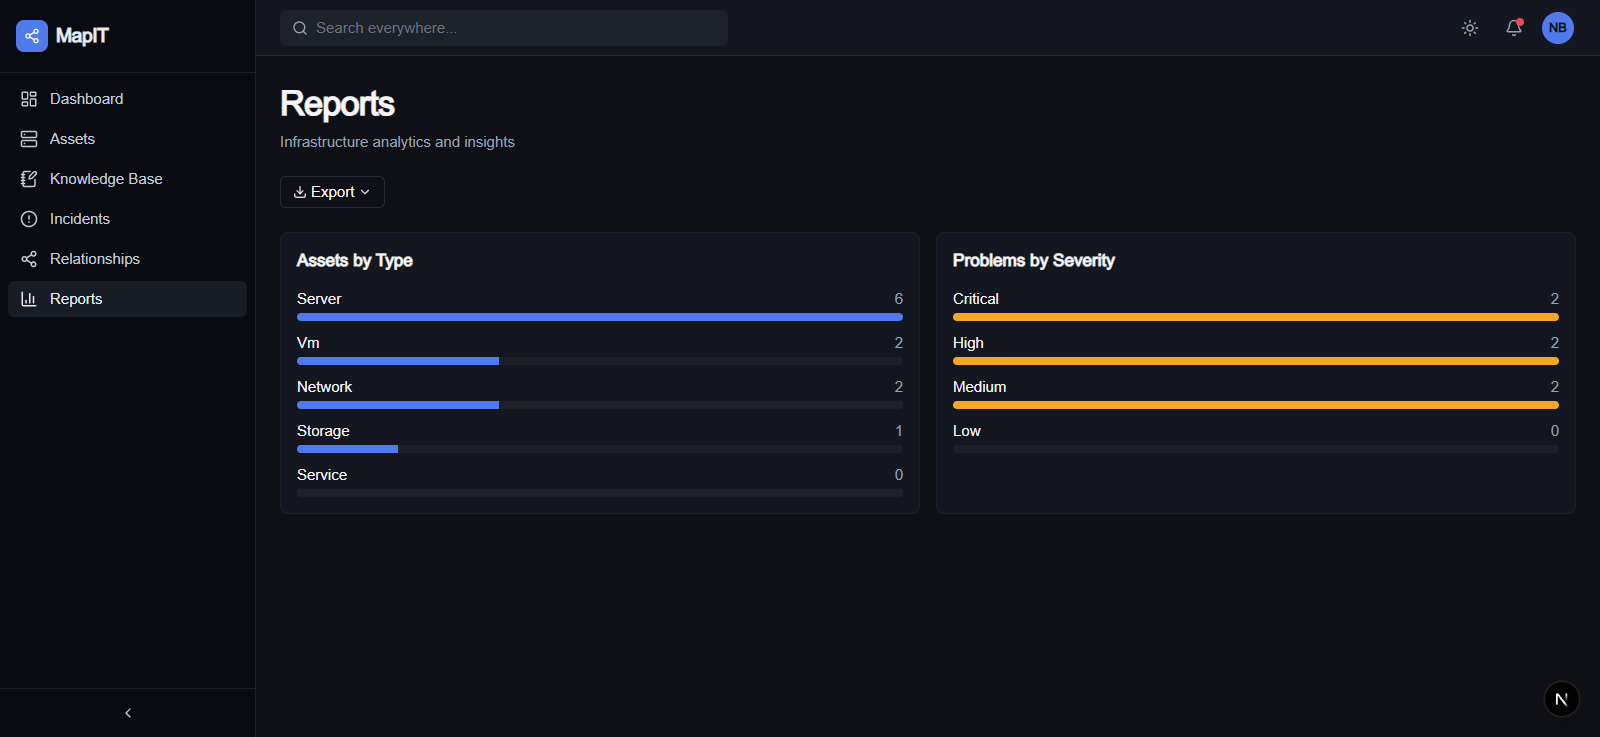
\includegraphics[width=0.95\textwidth]{figures/screenshots/reports.png}
	\caption{Reports interface}
	\label{fig:ui-reports}
\end{figure}

\section{Deployment and Execution Notes}
\subsection{Local execution}
The local development workflow is explicit: \texttt{npm run dev:api} starts the API on port 3000, \texttt{npm run dev:web} starts the web app on port 3001, and the root scripts support linting, type checking, integration testing, and smoke testing. This is consistent with the way the application is meant to be maintained during development.

\subsection{Environment and configuration}
The backend requires \texttt{DATABASE\_URL}, \texttt{JWT\_SECRET}, \texttt{AD\_URL}, \texttt{AD\_DOMAIN}, \texttt{CORS\_ORIGIN}, \texttt{ADMIN\_USERNAMES}, and \texttt{DEV\_MODE}. The web layer uses the proxy base \texttt{/api/backend} and the session route \texttt{/api/auth/session}. These configuration points are evidence that the project is already organized for a real deployment scenario.

\subsection{Production orientation}
The README describes deployment readiness on Vercel for the web application, Docker for the API, and Expo builds for the mobile prototype. The implementation chapter should therefore present MapIT as a deployable system rather than as a code-only exercise.

\section{Validation and Testing}
\subsection{Backend checks}
The backend uses integration tests under the Node test runner, and Prisma generation is part of the backend lifecycle. The audit logger, permission middleware, and authentication route can all be exercised through API requests, which is a strong basis for validation.

\subsection{Frontend checks}
The web app supports TypeScript type checking, linting, Playwright end-to-end testing, and smoke-style validation. These checks are useful because MapIT’s value depends not only on the backend data model but also on whether users can navigate the real pages effectively.

\section{Chapter Conclusion}
The implementation of MapIT is specific, structured, and aligned with the project’s academic objective. It combines a secure backend, a modern web frontend, a normalized data model, graph-based relationship mapping, global search, reporting, and access control. The next and final chapter can now synthesize the contribution of the project and outline future improvements.
